\chapter{Exam Questions}

\definecolor{backcolour}{rgb}{0.95,0.95,0.92}


\section{What is product-based software engineering?}

\textbf{Product-based software engineering} refers to the approach and methodology used in the development of software products. Unlike project-based development, where the primary focus is on delivering a specific solution for a client, product-based development centers around creating software that will be marketed, sold, and used by a broader audience. In product-based software engineering, the same company is responsible for deciding on both the features that should be part of the product and the implementation of these features;
customers, even if considered, do \textbf{not} decide on software features, releases or attributes, which is entirely up to the developer.
\begin{figure}[ht]
   \centering
   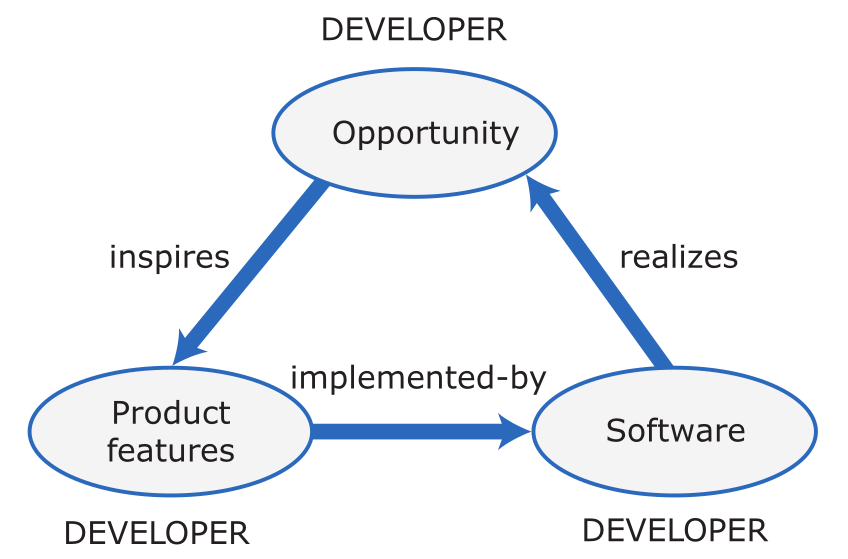
\includegraphics[width=0.5\linewidth]{images/questions/product-based-se.png}
   \caption{product based software engineering cycle}
   \label{fig:product-based-se}
\end{figure}
As showed above:
\begin{itemize}
   \item Because the product developer is responsible for identifying the \textbf{opportunity}, they can decide on the \textbf{features} that will be included in the software product. These features are designed to appeal to potential customers so that there is a viable market for the software. The product manager must ensure that development team implements features that deliver real value to customers.
         \note{In order to do so, he should regularly \textit{communicate with customers}, \textit{monitor technology constraints} relevant for customers, and keep the \textit{focus on goals} of both company and customers;
            in practice, this translates to
            \begin{itemize}[parsep=0em,topsep=0em,noitemsep]
               \tiny
               \item Product roadmap - goals, milestones, success criteria
               \item User stories and scenarios
               \item Product backlog (is product $manager \neq owner$?)
               \item Acceptance testing - verify that release meets set goals
               \item Customer testing
               \item Monitor usability in UI design
            \end{itemize}}
   \item Product companies can decide when to change their product or take their product off the market. The software developer decides also the platforms on which the software will be implemented, and so on.
\end{itemize}

\note{
   Product-based SE addresses the problem of mutable requirements which is becoming more and more common, crippling most Project-based software from early development stages.\\
   Two key differences from Project-based SE are:
   \begin{enumerate}[noitemsep]
      \item Quick software delivery is critical
      \item Software development starting point is the \textit{product vision}, i.e.
            \begin{itemize}[parsep=0em,topsep=0em,noitemsep]
               \tiny
               \item FOR target customer
               \item WHO need or opportunity
               \item THE product name is a product category
               \item THAT key benefit, compelling reason to buy
               \item UNLIKE primary competitive alternative
               \item OUR PRODUCT primary differentiation
            \end{itemize}
      \item \textbf{Prototyping} is the foundation of whole product development process,
            opposed to a project defined in advance.
      \item Customers, even if considered, do \textbf{not} decide on software features, releases or attributes, which is entirely up to the developer.
   \end{enumerate}
}

\section{What is the incremental development and delivery advocated by Agile? What are the key Scrum practices?}

\subsection{Incremental development and delivery}
\textbf{Incremental development and delivery} consists in breaking down the software development process into a set of features, with each doing something for the user, allowing developers not to worry about the details of all the features, you define only the details of the features that you plan to include in an increment.
\note{The features are prioritized in a way so that the most important features are implemented first}
Activities of incremental development typically are:
\begin{itemize}
   \item \textbf{Choose features to be included in an increment}: Using the list of features in the planned product, select those features that can be implemented in the next product increment.

         \note{
            Features with high priority should be preferred over others.
         }
   \item \textbf{Refine feature descriptions}: Add detail to the feature descriptions so that the team members have a common understanding of each feature and there is sufficient detail to begin implementation.
   \item \textbf{Implement and test}: Implement the feature and develop automated tests for that feature that show that its behavior is consistent with its description.
   \item \textbf{Integrate feature and test}: Integrate the developed feature with the existing system and test it to check that it works in conjunction with other features.
   \item \textbf{Deliver system increment}: Deliver the system increment to the customer or product manager for checking and comments. If enough features have been implemented, release a version of the system for customer use.
\end{itemize}
\subsection{Key Scrum practices}
\textbf{Scrum} is a lightweight framework that helps people, teams and organizations to create value through adaptive solutions to complex problems.
In Scrum, the software product is developed in a series of sprints, each of which delivers an \textbf{increment} of the product or supporting software. The Key Scrum practices are the following:
\note{These can be used in any agile development process even if other Scrum aspects are not applied.}
\begin{description}
   \item[Product backlog]: This is a to-do list of items {---}\textit{features(/user stories), engineering improvements, tools assessment} and other \textit{process activities}{---} to be implemented that is reviewed and updated before each sprint. Items in the product backlog are:
         \begin{itemize}
            \item ready for consideration
            \item ready for refinement
            \item ready for implementation
         \end{itemize}
         product backlog activities are:
         \begin{itemize}
            \item \textbf{refinement}: Existing PBIs are analysed and refined to create more detailed PBIs. This may lead to the creation of new product backlog items.
            \item \textbf{estimation}: The team estimate the amount of work required to implement a PBI and add this assessment to each analysed PBI. It is expressed in person-hours or person days or arbitrary "story points".
            \item \textbf{creation}: New items are added to the backlog, possibly suggested by the product manager.
                  \note{Even if called "features" in the Scrum lecture slides, they are typically expressed as \textit{user stories}.
                     \begin{center}
                        \emph{As a teacher, I want to be able to configure the group of tools that are available to individual classes. ({feature} / \emph{user story})}
                        (Ref. Slide 13)
                     \end{center}
                  }
            \item \textbf{prioritization}: The product backlog items are reordered to take new information and changed circumstances into account.
         \end{itemize}
   \item[Timeboxed sprints]: Fixed-time (2-4 week) periods in which items from the product backlog are implemented;
         The main sprint activities are:
         \begin{itemize}
            \item \textbf{Sprint planning}: Work items to be completed in that sprint are selected and, if necessary, refined to create a sprint backlog. This should not last more than a day at the beginning of the sprint.
            \item \textbf{Sprint execution}: The team work to implement the sprint backlog items that have been chosen for that sprint. If it is impossible to complete all of the sprint backlog items, the sprint is not extended. The unfinished items are returned to the product backlog and queued for a future sprint.
                  Usually during sprints two agile activities are used:
                  \begin{description}
                     \item[test automation]: As far as possible, product testing should be automated. You should develop a suite of executable tests that can be run at any time.
                     \item[continuous integration]: Whenever anyone makes changes to the software components they are developing, these components should be immediately integrated with other components to create a system. This system should then be tested to check for unanticipated component interaction problems.
                  \end{description}
            \item \textbf{Sprint reviewing}: The work done in the sprint is reviewed by the whole team and (possibly) external stakeholders. The team reflect on what went well and what went wrong during the sprint with a view to improving their work process. The product owner has the ultimate authority to decide whether or not the goal of the sprint has been achieved. They should confirm that the implementation of the selected product backlog items is complete.
         \end{itemize}
   \item[Self-organizing teams]: Self-organizing teams make their own decisions and work by discussing issues and making decisions by consensus (ideal size between 5 and 8 people), without a project manager. The advantage of a heterogeneous self-organizing team, where speech communication is preferred over work documentation amongst team members, is that it can be a cohesive team that can adapt to change.
         \note{
            In a Scrum project, the Scrum Master and the Product Owner should be jointly responsible for managing interactions with people outside the team.\\
            Scrum assumes that teams share a workspace and that all team members can attend a morning meeting to coordinate the work for the day.}
\end{description}

\section{What are personas, scenarios, user stories, and features?}
\begin{itemize}
   \item \textbf{Personas} are (imaginary) types of product users. They are used to understand potential users in order to design features that will be useful to them. They give background, skills and experience of potential users. Personas allow developers to "step into the users' shoes".
         \note{Usually only a couple of personas (max 5) are needed to identify key product features.

            They should include personal, education and job-related information, along with other details which may indicate their interest in the product}
   \item \textbf{Scenarios} are narratives describing a situation in which a user is using our product's features to do something he/she wants to do. High-level scenarios facilitate communication and stimulate design creativity. Scenarios are not specifications, so they lack detail and may be incomplete. They are written from the user's perspective (3-4 for each persona).
         \note{They should be created by every team member and discussed together, possibly also with customers.

            Even though it is possible to express all functionalities described in a \textit{scenario} using \textit{user-stories},
            scenarios can read more naturally, make stories understanding easier, and provide more context.}
   \item \textbf{User stories} are finer-grained narratives that describe, in a more detailed and structured way, "a single what" a user wants from a software system. The standard format of a user story is:

         As a $<role>$, I $< want / need>$ to $<do$ $something>$

         \note{They allow to organize and chunk work into single units which represent actual value to the customer, ultimately building software incrementally from the users perspective.
            A story which involves multiple sprints to be implemented (hence is in some sense "longer") is called an "\textbf{epic}",
            and can be split into shorter stories.
            An example of an epic may be:
            \begin{center}
               \textit{"\textbf{As a} system manager, \textbf{I need} a utility tool \textbf{to} back up and restore individual applications, files, or the whole system"}
            \end{center}}

         \note{Usually a \textit{Scrum product backlog} is a set of \textit{user stories} sorted according to priority.}

   \item A \textbf{feature} is a way for users to access and use the functionality of your product, so the feature list defines the overall functionality of the system. The properties of the features are shown below:
         \begin{itemize}
            \item \textit{independence}: a feature should not depend on how other system features are implemented and should not be affected by the order of activation of other features
            \item \textit{coherence}: features should be linked to a single item of functionality and not have side effects
            \item \textit{relevance}: system features should reflect the way users normally carry out some task, rather than introducing obscure or rarely needed functionality
         \end{itemize}
         \note{They should result from combining User Knowledge (expressed as User Stories/Personas/Scenarios), Domain, Product and Technology knowledge}
\end{itemize}


\section{What is the role of non-functional quality attributes and decomposition in a software architecture? What is a distribution architecture? What are the technology choices that affect a software architecture? What are the main features of Enterprise Integration Patterns?}
\subsection{Non-functional quality attributes and decomposition}
\textbf{Non-functional quality attributes} have the role to describe aspects of a software system that are not related to its specific functionalities but are crucial for evaluating its overall performance. These attributes are critical to the final product, but not to the prototype.
\note{Note that optimizing one non-functional attribute might affect others}
Non-functional quality attributes are:
\begin{itemize}

   \item\textbf{responsiveness}: Does the system return results to users in a reasonable time?
   \item\textbf{reliability}: Do the system features behave as expected by both developers and users?
   \item\textbf{availability}: Can the system deliver its services when requested by users?
   \item\textbf{security}: Does the system protect itself and users’ data from unauthorized attacks and intrusions?
   \item\textbf{usability}: Can system users access the features that they need and use them quickly and without errors?
   \item\textbf{maintainability}: Can the system be readily updated and new features added without undue costs?
   \item\textbf{resilience}: Can the system continue to deliver user services in the event of partial failure or external attack?
\end{itemize}


\textbf{Decomposition} increases the maintainability of the system by decomposing the system into small \textbf{self-contained} parts: $Service < Component < Module$ where \textit{Service} is a coherent unit of functionality, and the \textit{Component} a unit providing a set of related services.
Too much decomposition increases the complexity of the architecture, and consequently the integration between components. Good practices to control the complexity are:
\begin{itemize}
   \item \textbf{separation of concerns}: organize your architecture into components that focus on a single concern;
   \item \textbf{stable interfaces}: design interfaces that are coherent and that change slowly;
   \item \textbf{implement once}: avoid duplicating functionality at different places in your architecture.
\end{itemize}
\note{\begin{itemize}[parsep=0em,noitemsep,topsep=0em]
      \item \textbf{Localize relationships} between components by putting them in the same module
      \item \textbf{Avoid data sharing} among components
   \end{itemize}}
\note{Despite implying a mixup between implementation and design, system decomposition must be done in conjunction with choosing technologies for the system.}
\subsection{Distribution architecture}
A \textbf{distribution architecture} (figure \ref{fig:client-server}) defines servers and allocation of components to servers. For example, client–server architectures are a type of distribution architecture that is suited to applications in which clients access a shared database and business logic operations on those data.

These applications include several servers, such as web servers and database servers. Access to the server set is usually mediated by a load balancer, which distributes requests to servers. It is designed to ensure that the computing load is evenly shared by the set of servers.

\begin{figure}[ht]
   \centering
   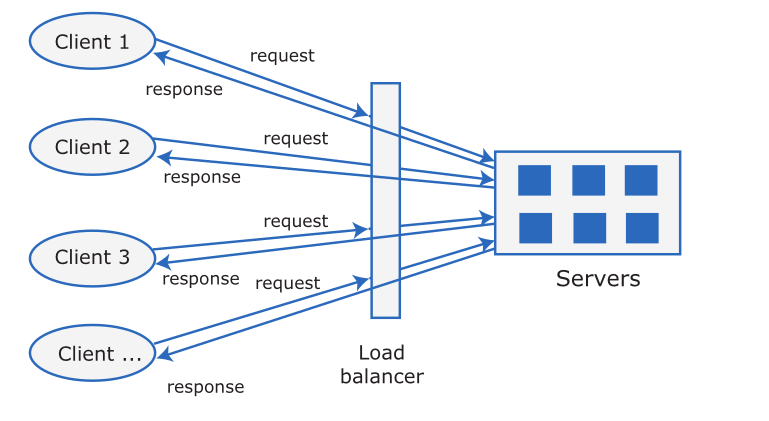
\includegraphics[width=0.5\linewidth]{images/questions/client-server.png}
   \caption{client-server architecture}
   \label{fig:client-server}
\end{figure}
The majority of software products are now web-based products, so they have a client-server architecture, usually based on the \textbf{Model-View-Controller (MVC) pattern}.
The term \textit{model} is used to mean the system data and the associated business logic. and is shared and maintained on the server.
Each client has its own updated view of the data, with the controller (residing on the client-side) acting as an intermediary.

\begin{figure}[ht]
   \centering
   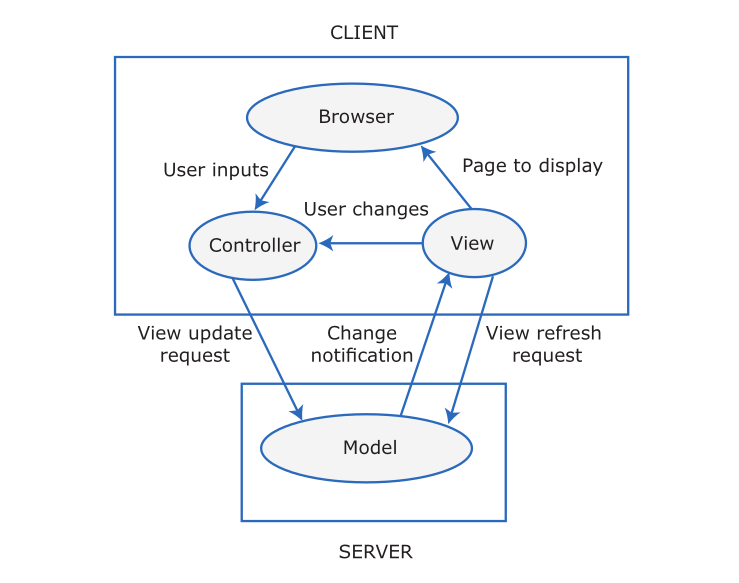
\includegraphics[width=0.5\linewidth]{images/questions/MVC.png}
   \caption{mvc pattern}
   \label{fig:mvc}
\end{figure}
Many web-based applications use \textbf{a multi-tier architecture} with several communicating servers, each with its own responsibilities.
\begin{figure}[ht]
   \centering
   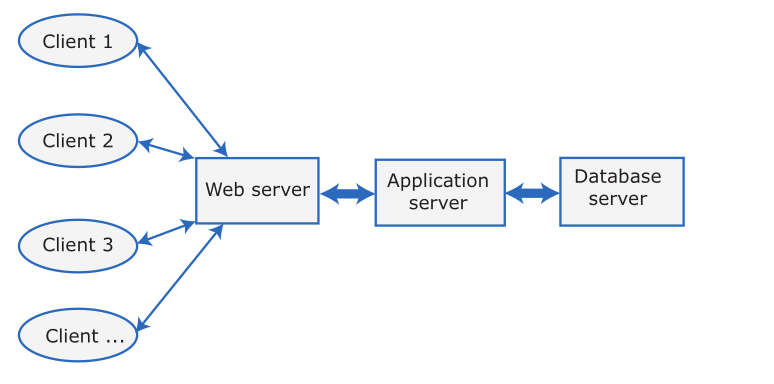
\includegraphics[width=0.5\linewidth]{images/questions/multi-tier.png}
   \caption{multi-tier client-server architecture}
   \label{fig:multi-tier}
\end{figure}

An alternative to a multi-tier client–server architecture is a \textbf{service-oriented architecture} where many servers may be involved in providing services. Services in a service-oriented architecture are stateless components, which means that they can be replicated and can migrate from one computer to another. A service-oriented architecture is usually easier to scale as demand increases and is resilient to failure.
Multi-tier and service-oriented architectures are the main types of distribution architecture for web-based and mobile systems. You have to decide which of these to choose for your software product.
\begin{figure}[ht]
   \centering
   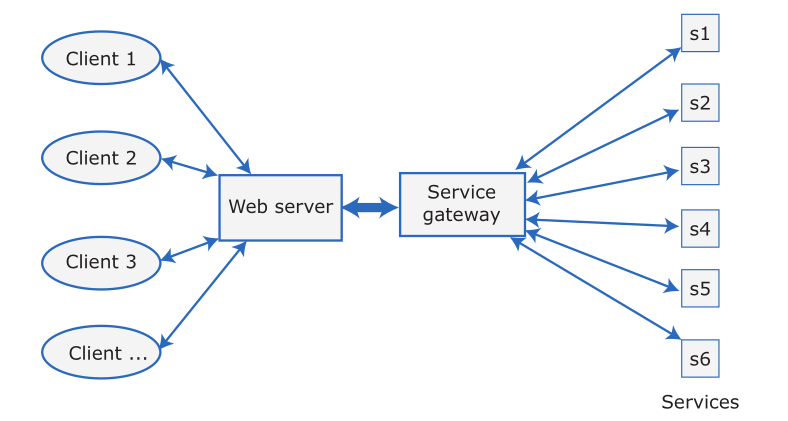
\includegraphics[width=0.5\linewidth]{images/questions/service-oriented.png}
   \caption{service oriented architecture}
   \label{fig:service oriented}
\end{figure}
Factors that influence what architecture to choose are:
\begin{itemize}
   \item \textbf{Data type and data updates}: If you are mostly using structured data that may be updated by different system features, it is usually best to have a single shared database that provides locking and transaction management. If data are distributed across services, you need a way to keep them consistent, and this adds overhead to your system.
   \item \textbf{Change frequency}: If you anticipate that system components will regularly be changed or replaced, then isolating these components as separate services simplifies those changes.
   \item \textbf{The system execution platform}: If you plan to run your system on the cloud with users accessing it over the Internet, it is usually best to implement it as a service-oriented architecture because scaling the system is simpler. However, if your product is a business system that runs on local servers, a multi-tier architecture may be more appropriate.
\end{itemize}

\subsection{Technologies choices}
The \textbf{technologies choices} that affect and constrain the overall system architecture and that are difficult/expensive to change during the development are:
\begin{itemize}
   \item \textbf{database}: should you use a relational SQL database or an unstructured NoSQL database?
   \item \textbf{platform}: should you deliver your product on a mobile app and/or a web platform?
   \item \textbf{server}: should you use dedicated in-house servers or design your system to run on a public cloud? If a public cloud, should you use Amazon, Google, Microsoft, or some other option?
   \item \textbf{open source}: are there suitable open-source components that you could incorporate into your products?
   \item \textbf{development tools}: do your development tools embed architectural assumptions about the software being developed that limit your architectural choices?
\end{itemize}

\subsection{Enterprise Integration Patterns}
An EIP is a reusable abstraction of proven solutions to well-known problems that arise when integrating the software components/services that make up enterprise applications.

They mainly address the problem of handling the communication between services, data sources and participants.
The foundation of the integration achieved by EIPs are one-way channels (point-to-point or publish-subscribe) and message endpoints, but may be enriched by various other components, such as
\begin{enumerate}[parsep=0em,noitemsep,topsep=0em]
   \item \begin{enumerate}
      \item \textit{Adapters} - Application to Channel
      \item \textit{Translators} - Format suitable for receivers
      \item \textit{Normalizers} (Router+Translators) - Normalizing data coming from multiple sources in various formats in a single output 
      \item \textit{Content Enrichers} - Add context info to messages
   \end{enumerate}
   \item 
   \begin{enumerate}
      \item \textit{Routers} - Route messages to desired receivers
      \item \textit{Splitters} - Duplicate/split message to multiple receivers
      \item \textit{Aggregators} - Aggregate messages coming from multiple sources, blocking until all messages are received
   \end{enumerate}
\end{enumerate}

\section{What is a Docker image/container? What is Docker Compose? What are the differences between multi-tenant and multi-instance SaaS systems? What are the design principles of K8s? How does K8s control plane work?}

\subsection{Docker}
\begin{itemize}
   \item A \textbf{docker container} is a standalone and executable software package that includes everything needed to run a piece of software, including the code, runtime, libraries, and system tools.
         \note{Unlike VMs container-based virtualization does not require emulating an entire OS}
         Docker containers are based on images and can be started, stopped, moved, and deleted independently of the underlying infrastructure.
   \item An \textbf{docker image} is a software component which is exploited as read-only templates to create and run containers. images are built from a set of instructions (using a Dockerfile) and include a snapshot of the application and its dependencies. images are stored in a (private or public) Docker registry (e.g. Docker Hub).
   \item \textbf{Docker Compose} is a tool to define and run multi-container Docker applications. It allows you to define an entire application stack, including services, networks, and volumes, in a single file, named docker-compose.yml. All services defined in the file can be started with the command \textit{docker-compose up}. It simplifies the process of managing multiple containers that need to work together as part of a larger application.
\end{itemize}

\subsection{Multi-tenant vs multi-instance}
The difference between multi-tenant and multi-instance systems is that:

multi-tenant systems use a single database schema shared by all system's users. The items in database are tagged with tenant identifier to provide "logical isolation", so that customer companies have their
own space and can store and access their own data.
\note{Mid-size and large businesses usually want a version of the multi tenant software
   that is adapted to their own requirements}
\begin{figure}[ht]
   \centering
   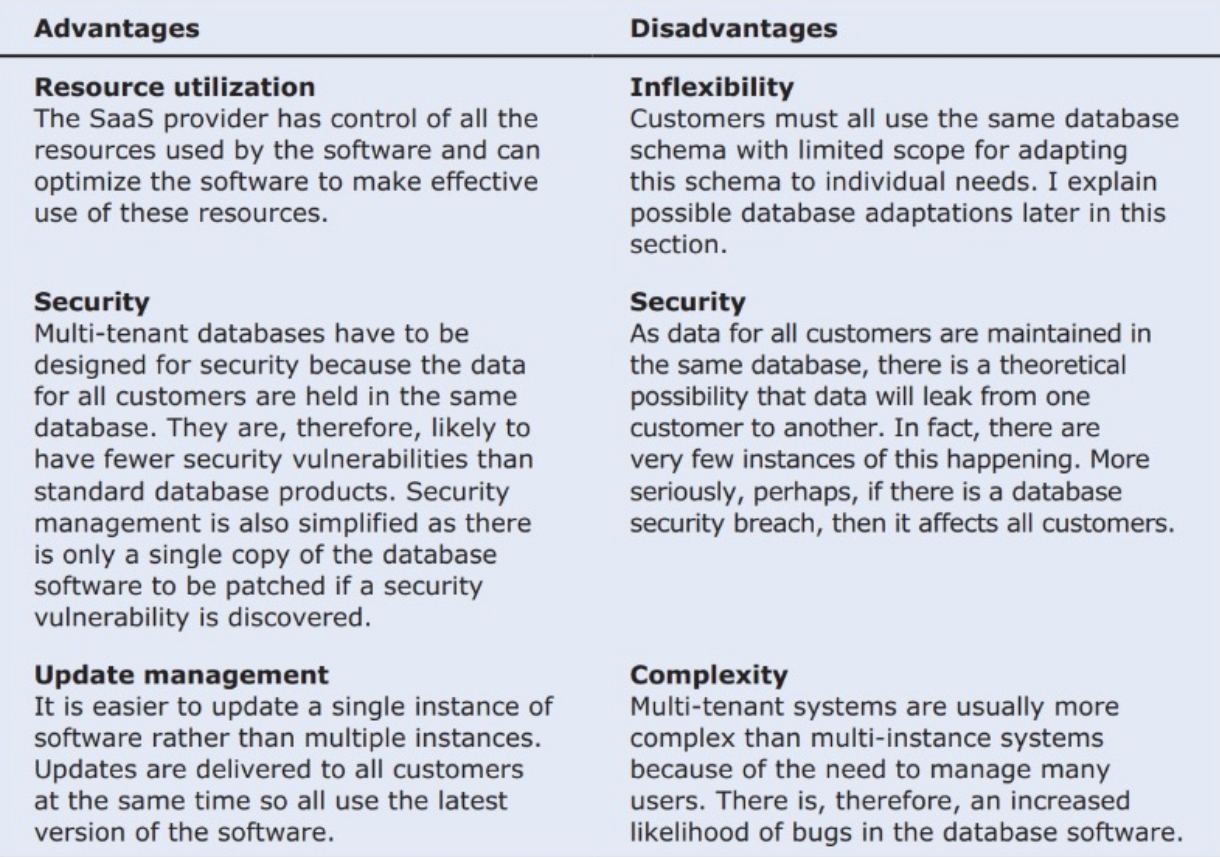
\includegraphics[width=0.5\linewidth]{images/questions/multi-tenant.png}
   \caption{pros and cons of multi-tenant}
   \label{fig:multi-tenant}
\end{figure}
multi-instance systems means that each customer has its own system tailored to its needs, including its own database and security controls. It can be VM-based or Container-based (also you can run multiple containers for individual users on top of a VM-based system).
\begin{figure}[ht]
   \centering
   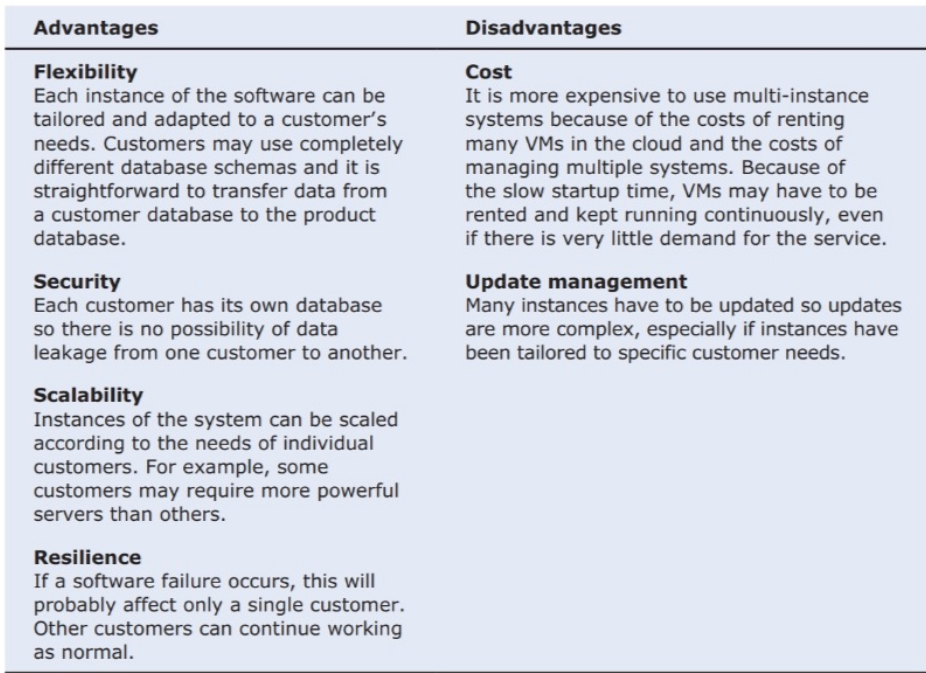
\includegraphics[width=0.5\linewidth]{images/questions/multi-instance.png}
   \caption{pros and cons of multi-instance}
   \label{fig:multi-instance}
\end{figure}
Conceptually a multi-instance system in simpler than a multi-tenant system and avoids concerns such as inter-organization data leakage.

\note{
   Let's consider \textit{pros and cons} of such a solution.
   Flexibility, security, scalability and resilience are clearly some key points of \textit{multi-instance DBs}.
   However update management difficulty and cloud VMs renting costs are not negligible.

   Wrapping up,
   there are three possible ways of
   providing a customer \textbf{database} in
   a \textit{cloud-based} system:
   \begin{enumerate}
      \item As a \textbf{multi-tenant} system, \textit{shared by all customers} for your product.
            This may be hosted in the cloud using large, powerful servers.
      \item As a \textbf{multi-instance} system, with \textit{each customer database} running on its own \textit{virtual machine}.
      \item As a \textbf{multi-instance} system, with \textit{each database} running in its own \textit{container}.
            The customer database may be distributed over several containers.
   \end{enumerate}
}

\subsection{K8s}
The design principles of K8s are:
\begin{itemize}
   \item \textbf{declarativeness}: we simply define the desired state of our system and K8s will detect when the actual state of the system doesn't meet our expectations and it will intervene to fix the problem, making our system self-healing. The desired state is defined by a collection of objects, each of which has a specification in which you specify the desired state and a status that reflects the current state of the object. K8s constantly polls each object to ensure that its status is equal to the specification (e.g. if an object is unresponsive, K8s will spin up a new version to replace it).
   \item \textbf{distribution}: K8s provides a unified interface for interacting with a cluster of machines. We don't have to worry about communicating with each machine individually.
   \item \textbf{decoupling}: Containers should be developed with a single concern in mind (implements a microservice-based architeture). K8s naturally supports the idea of decoupled services which can be scaled and updated independently.
   \item \textbf{immutable infrastructure}: to get the most out of containers and container orchestration, we should use an immutable infrastructure. During the life-cycle of a project (development - testing - production) we should use the same container image. Containers are designed to be ephemeral, ready to be replaced by another container instance at any time. Maintaining immutable infrastructure makes it easier roll back applications to previous state (eg. if an error occurs) - we can simply update our configuration to use an older container image.
\end{itemize}
The K8s control plane relies on the \textbf{master node}: (often unique) machine that contains most of the control plane components:
\begin{itemize}
   \item The user provides new/updated object specification to \textbf{API server}(figure \ref{api-server}) of master node, then API server validates update requests and acts as unified interface for questions about cluster's current state. The state of cluster is stored in a distributed key-value store etcd, a distributed key-value store.
         \begin{figure}[ht]
            \centering
            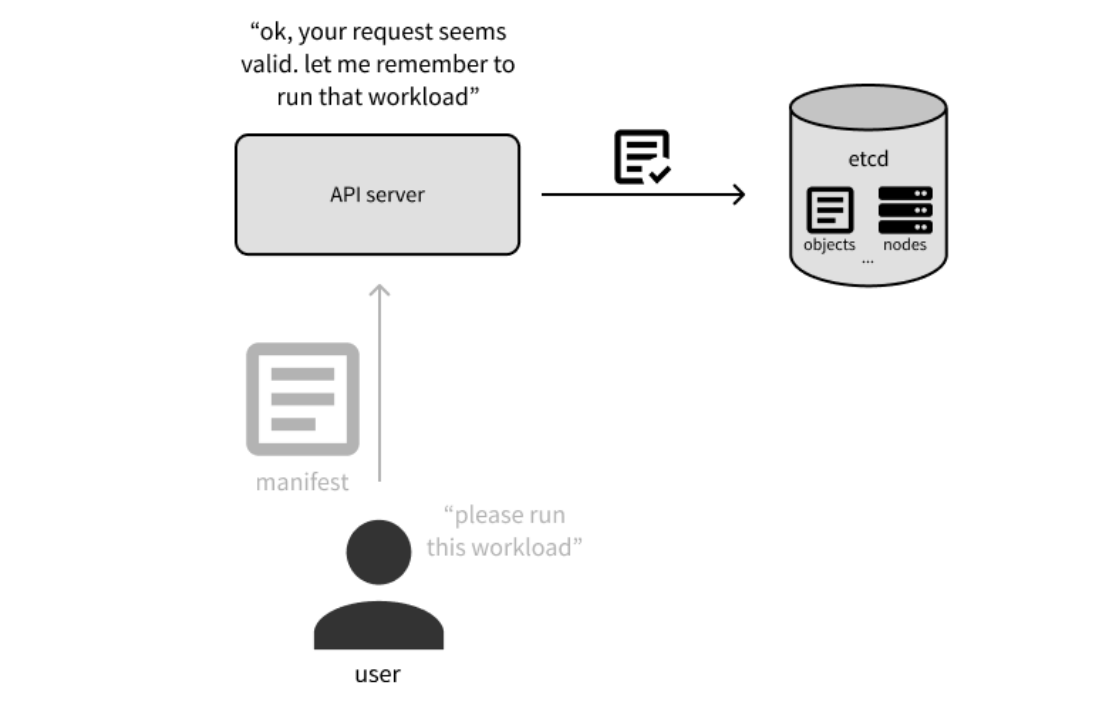
\includegraphics[width=0.5\linewidth]{images/questions/api-server.png}
            \caption{api server of the master node.}
            \label{api-server}
         \end{figure}
   \item The \textbf{scheduler}(figure \ref{scheduler}) determines where to run objects by asking the API server which objects have not been assigned to a machine, determining which machines those objects should be assigned to, and responding back to the API server to reflect this assignment.
         \begin{figure}[ht]
            \centering
            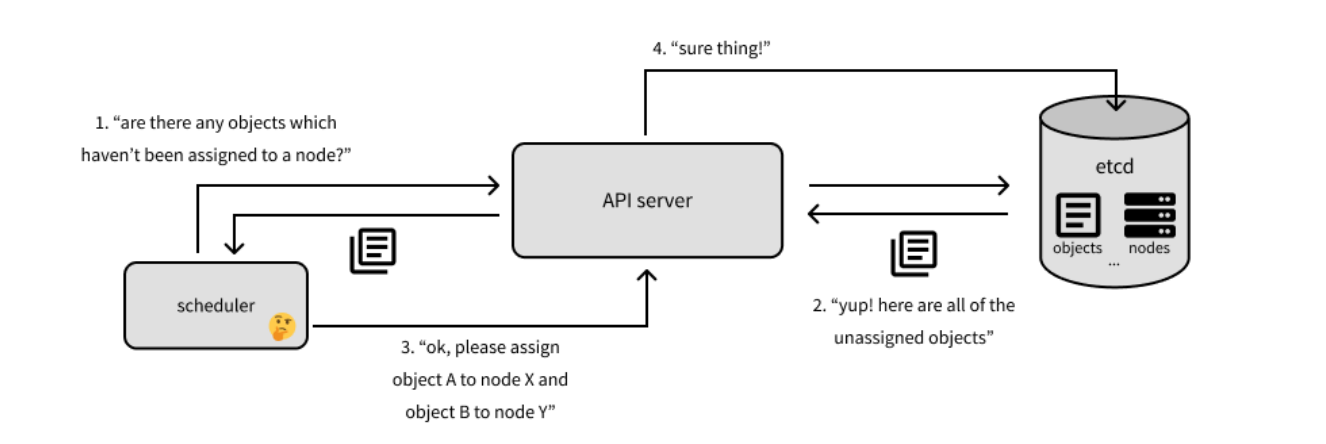
\includegraphics[width=1\linewidth]{images/questions/scheduler.png}
            \caption{scheduler of the master node.}
            \label{scheduler}
         \end{figure}
   \item The \textbf{controller-manager}(figure \ref{controller-manager}) monitors cluster state through the API server. If actual state differs from desired state, the controller-manager will make changes via the API server to drive the cluster towards the desired state.
         \begin{figure}[ht]
            \centering
            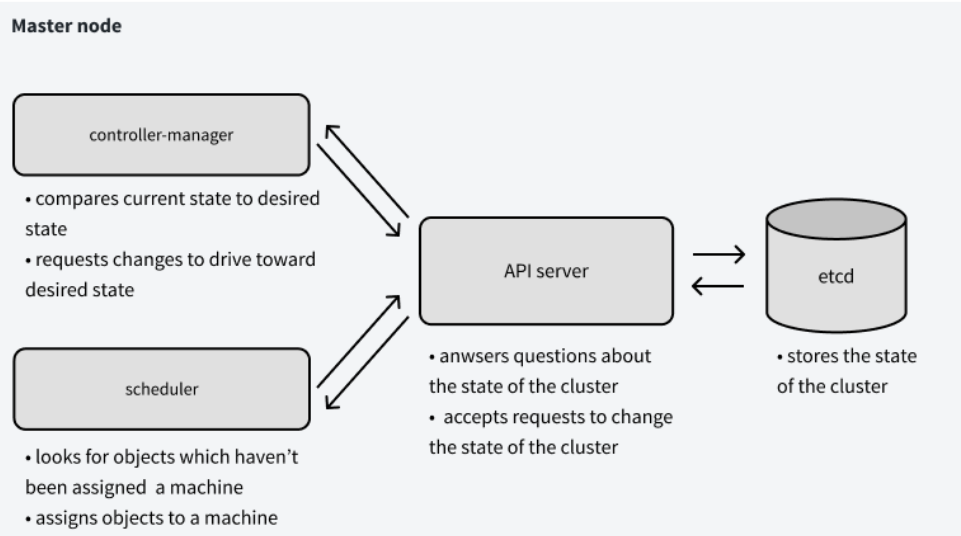
\includegraphics[width=0.75\linewidth]{images/questions/controller-manager.png}•
            \caption{controller manager of the master node.}
            \label{controller-manager}
         \end{figure}
\end{itemize}


\section{What are the main (dis)advantages and characteristics of microservices? What does the CAP theorem tell us? Which refactoring can be applied to resolve architectural smell X?}

\subsection{Microservices: characteristics, pro and cons}
Microservices are small-scale services that can be combined to create applications. They are independent (the service interface is not affected by changes to other services), allowing a service to be modified and redeployed without modified/stopping other services. \nl

The main characteristics of microservices are the following:
\begin{itemize}
   \item \textbf{self-contained}: microservices do not have external dependencies. They manage their own data and implement their own user interface.
         \note{User interface? }
   \item \textbf{lightweight}: microservices communicate using lightweight protocols so that service communication overhead is low.
         \note{Sacrifing the generality that’s inherent in the design of web service protocols}
   \item \textbf{independent implementation}: microservices may be implemented using different programming languages and may use different technologies (e.g. different types of database) in their implementation.
   \item \textbf{independently deployable}: each microservice runs in its own process and is independently deployable using automated systems.
   \item \textbf{business-oriented}: microservices implement business capabilities and needs, rather than simply provide a technical service.
\end{itemize}
The main two reasons (pro) to adopt microservices are:
\begin{enumerate}
   \item \textbf{Reduced lead time for new features and updates}: this is made possible by \textit{autonomous teams} working on different, independent and decoupled services, and \textit{continuous deployment}.
   \item \textbf{Scale}: it is effectively possible to scale up or down a service, e.g. in case of large amount of load, it is possible to deploy new replica to balance the load and avoid congestion.
\end{enumerate}
On the other hand there are also some cons, that are:
\begin{itemize}
   \item \textbf{communication overhead}: Microservices communicate with each other over a network. This can introduce latency and additional complexity, especially in cases where frequent communication is required between microservices.
   \item \textbf{complexity}: Coordinating and managing a large number of microservices can lead to challenges in understanding, deploying, and maintaining the entire system.
   \item \textbf{"wrong cuts"}: If the splitting of the monolothic application is done incorrectly, it may lead to suboptimal microservices that are either too coarse-grained or too fine-grained.
         \note{See also \textit{cohesion} and \textit{coupling}, regarding the number of intra/intercommunications.}
   \item \textbf{“avoiding data duplication as much as possible while keeping microservices in isolation is one of the biggest challenges”}
   \item \textbf{“A poor team will always create a poor system”}: Success with microservices relies heavily on collaboration, communication, and skilled teams. Inadequate team collaboration or lack of expertise can lead to poorly designed and implemented microservices.
         \note{The observation on teams impacts more than any microservices-over-monolith choice dictated by system complexity}
\end{itemize}

\subsection{CAP Theorem}
The CAP theorem says that "It is impossible for a web service to provide Consistency, Availability and Partition-tolerance at the same time", where:
\begin{itemize}
   \item \textbf{Consistency}: each service returns the "right" response to each request,
   \item \textbf{Availability}: each request eventually receives a response,
   \item \textbf{Partition-tolerance}: services can be partitioned into multiple groups, and network can delay/lose arbitrarily many messages among services.
\end{itemize}
\subsection{Architectural smell}
An architectural smell is a commonly used architectural decision that negatively impacts system lifecycle qualities. An architectural smell is a threat to one or more of these {---}microservices{---} design principles:
\begin{itemize}
   \item \textbf{Independent deployability}: The microservices forming an application should be independently deployable;
   \item \textbf{Horizontal scalability}: The microservices forming an application should be horizontally scalable;
   \item \textbf{Isolation of failures}: Failures should be isolated;
   \item \textbf{Decentralization}: Decentralization should occur in all aspects of microservice-based applications, from data management to governance.
\end{itemize}
There are several ways to resolve a smell by refactoring a microservice. During the course we saw MicroFreshener which is a tool which edits app specifications, automatically identifies architectural smells and allow the user to apply one of the suggested refactors to the architecture. Then, the application manager can implement concretely the refactoring modifying the code of the application.

\note{During the course we discussed which are the possible solutions for each architectural smell, which are the same that MicroFreshener proposes.
   They are summarized in the table below:
}
\begin{figure}[htbp]
   \centering
   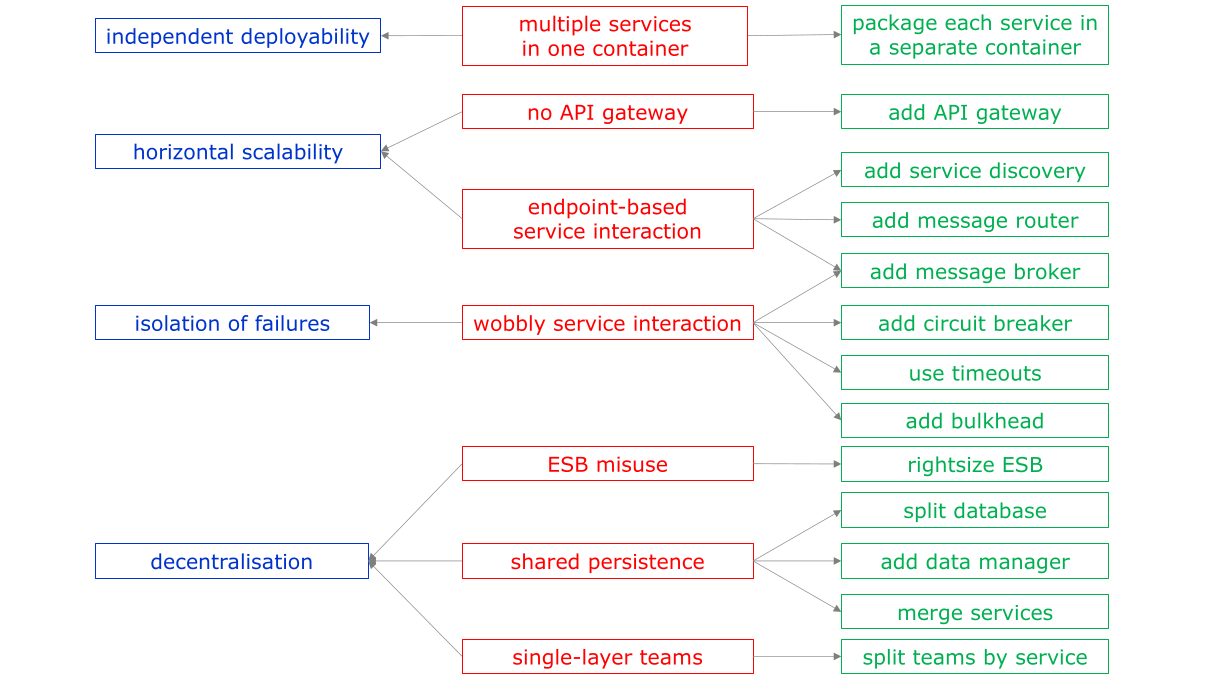
\includegraphics[width=0.8\textwidth]{images/questions/smells.png}
   \caption{Smells and corresponding solutions}
\end{figure}
\note{\begin{itemize}
   \item \textbf{Message broker}:  between services. This helps decouple services, improve fault tolerance, and enable event-driven architecture
   \item \textbf{Message router}:  route messages based on content, headers, or other criteria.
   \item \textbf{Bulkhead}: pattern indicating t use separate resources (e.g., databases, thread pools) for different microservices, preventing failures in one area from affecting others.
   \item \textbf{rightsize ESB}:
   \\textit{"ESB"} stands for Enterprise Service Bus, i.e. an architectural pattern whereby a centralized software component performs integrations between applications.\\
   An ESB designed for a monolithic architecture may become a bottleneck, $\longrightarrow$  break down its components into more lightweight and focused communication mechanisms. Consider replacing the monolithic ESB with more decentralized and targeted communication patterns, such as direct HTTP/REST calls or message brokering.
\end{itemize}}

\subsection*{Emiliano - Smells and refactoring}
All the \textcolor{red}{architectural smells} will be categorized based on the \textcolor{blue}{design principle} they violate. For each smell will be presented some \textcolor{green}{refactorings} to solve them.
\subsubsection{Independent deployability}
One \textit{architectural smell} for \textcolor{blue}{independent deployability} is \textcolor{red}{multiple services in one container} (because ideally we want to have one container per microservices). It is possible to insert some microservices that interact a lots inside the same container, but this can lead to various problems. The solution for this smell is to \textcolor{green}{package each service in a separate container}.

\subsubsection{Horizontal scalability}
One first \textit{architectural smell} for \textcolor{blue}{horizontal scalability} is \textcolor{red}{endpoint-based service interaction}. This is a smell because, in the case it's present an interaction to a specific service istance (as shown in Figure \ref{fig:end-point-img1}), adding more replicas of the service won't scale the application, since the interaction is made with only one of the replicas. Some \textit{refactoring} for the described \textit{smell} are to \textcolor{green}{add a service discovery} that will indicate to the requester which replica he must use (applied in the 55\% of cases), \textcolor{green}{add a message router} that will redirect the request to one of the replicas (e.g. load balancer, applied in the 31\% of cases) or \textcolor{green}{add a message broker} that will collect the requests, which are then collected from the replicas (e.g. message queue, applied in the 14\% of cases). The reason that the message broker is the least used is because the code of the microservice has to be modified.
\begin{figure} [H]    \centering
    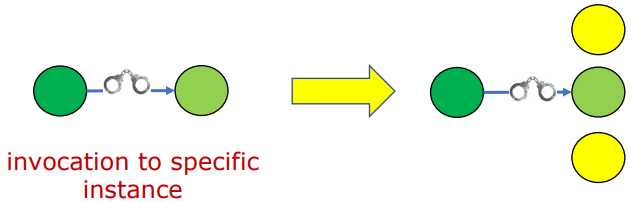
\includegraphics[width=0.65\textwidth]{images/end-point-img1.PNG}    \caption{Endpoint-based service interaction}
    \label{fig:end-point-img1}\end{figure} 
Another \textit{architectural smell} is the \textcolor{red}{absence of an API gateway}, because clients can invoke directly the services (it's similar to endpoint-based service interaction smell). The solution is simply to \textcolor{green}{add an API gateway}, since not only resolve the smell, but can also be useful also for authentication, throttling, and so on.
%\newpage 

\subsubsection{Isolation of failures}
One \textit{architectural smell} for \textcolor{blue}{isolation of failures} is \textcolor{red}{wobbly service interaction}: the interaction of m1 with m2 is \textit{wobbly} when a failure of m2 can trigger a failure of m1. Some \textit{refactoring} for the described \textit{smell} are to \textcolor{green}{add a circuit breaker} (applied in the 42\% of cases), \textcolor{green}{use timeouts} (applied in the 22\% of cases), \textcolor{green}{add a bulkhead} (applied in the 20\% of cases), or \textcolor{green}{add a message broker} (applied in the 16\% of cases).
\subsubsection{Decentralization}
One first \textit{architectural smell} for \textcolor{blue}{decentralization} is \textcolor{red}{shared persistence}. Three proposed solutions (that are better described with the Figure \ref{fig:shared_persistence}) are \textcolor{green}{split database} (applied in the 50\% of cases), \textcolor{green}{add data manager} that acts as a gateway between the services and the database (applied in the 22\% of cases) or \textcolor{green}{merge services} (applied in the 9\% of cases).
\begin{figure} [H]    \centering
    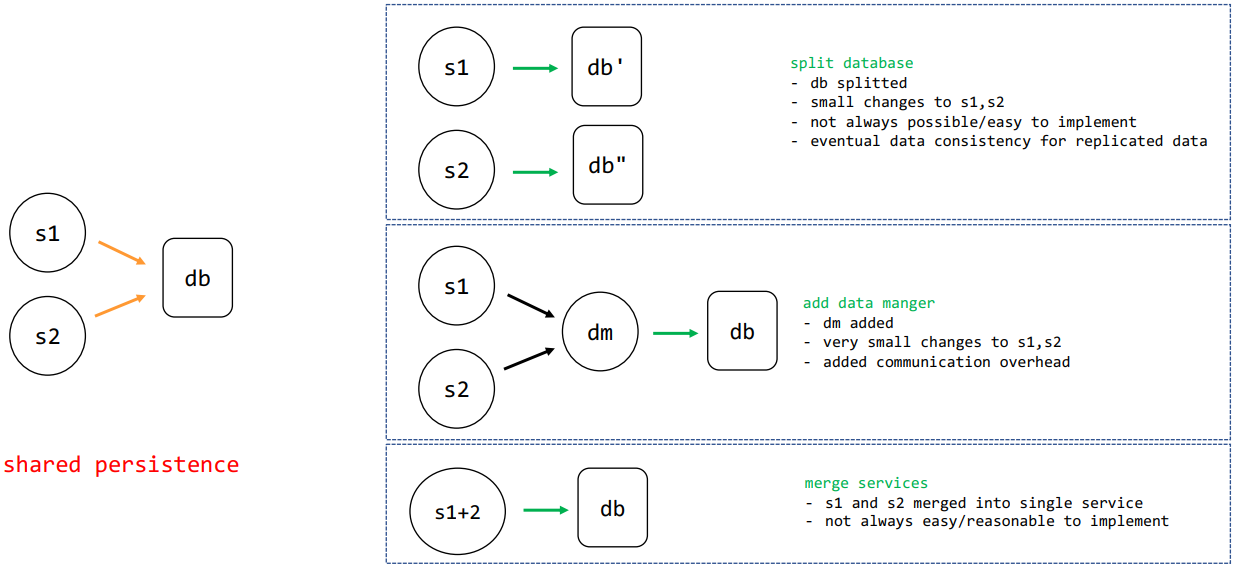
\includegraphics[width=1\textwidth]{images/shared_persistence.PNG}    \caption{Solutions for shared persistence}
    \label{fig:shared_persistence}\end{figure} 
The last \textit{architectural smell} is the \textcolor{red}{single-layer teams}, which goes in contrast to the idea of Agile. The solution is simply to \textcolor{green}{split teams by service}.


\section{How can we feature authentication and authorization in a software product? What are the main challenges in securing microservices?}
\subsection{Authentication in software product}
We can feature authentication in a software product with one of this approaches:
\begin{itemize}
   \item \textbf{Knowledge-based authentication}: it relies on users providing secret, personal information at registering time;
   \item \textbf{Possession-based authentication}: it relies on users having a physical device that can be connected to the authentication system and that generates/displays information known to the authentication system (e.g. system sends code to user’s phone number, or special-purpose device that generates one-time codes);
   \item \textbf{Attribute-based authentication}: it relies on a unique biometric attribute of the user (e.g. fingerprint, face).
\end{itemize}
Nowadays many systems now use multi-factor authentication, which is the combination of two or more of the types shown above (e.g. password, then code received on mobile phone).

Knowledge-based authentication often employed for products delivered as
cloud services.

\note{Some services provide a \textbf{federated} authentication method e.g. \textit{"Login with Google"}, typically implemented using library \texttt{OAuth},
   which rely on a trusted third party authenticator;}

Weaknesses of password-based authentication
\begin{itemize}
   \item Users choose insecure passwords that are easy to remember
   \item Users click on email link pointing to fake site that collects login and password → phishing attack
   \item Users use the same password for several sites (if there is a security breach at one site …)
   \item Users regularly forget passwords → password recovery mechanism needed → potential vulnerability if credentials have been stolen.
\end{itemize}
defenses
\begin{itemize}
   \item Force users to set strong passwords
   \item Add personal questions
\end{itemize}

The level of authentication that you need depends on your product
\begin{itemize}
   \item No need to store confidential user information → knowledge-based authentication enough
   \item Need to store confidential user information → use two-stage authentication
\end{itemize}

Implementing a secure and reliable authentication system is expensive and time-consuming
\begin{itemize}
   \item Even if using available toolkits and libraries (e.g. OAuth), there is still a lot of programming effort involved
   \item Authentication often outsourced with a \textbf{federated identity system}
\end{itemize}
Sometimes websites offer the opportunity to “Login with Google” or “Login with Facebook.” These sites rely on what is called a “federated identity” approach, where an external service is used for authentication.

the advantages of this approach are:
\begin{itemize}
   \item user has single set of credentials, stored by a trusted identity service
   \item product provider doesn’t have to maintain own database of passwords/secrets
   \item product provider can get additional user information (if user agrees)
\end{itemize}
disadvantages: product provider must share user information with external services.

Federated identity verification is ok for products aimed at individual customers and for business products, connecting to business' own identity management system.

There are various ways to implement federated authentication, but most of the major companies that offer federated authentication services use the OAuth protocol. This standard authentication protocol has been designed to support distributed authentication and the return of authentication tokens to the calling system.
(bonus part from the book)

However, OAuth tokens do not include information about the authenticated user. They only indicate that access should be granted. This means it is not possible to use OAuth authentication tokens to make decisions on user privileges (for example, what resources of the system they should have access to). To get around this problem, an authentication protocol called OpenID Connect has been developed that provides user information from the authenticating system. Most of the major authentication services now use this, except Facebook, which has developed its own protocol on top of OAuth.

\subsection{Authorization in software product}
We can feature authorization by using an \textbf{access control policy} that reflects data protection rules that limit access to personal data. \textbf{Access Control Lists (ACLs)} are widely used to implement acces control policies. ACLs classify individuals into groups dramatically reducing ACLs size. Different groups can have different rights on different resources. Hierarchies of groups allow to assign rights to subgroups/individuals. ACLs are often realized by relying on ACL of underlying file or database system.

\note{Since containers are stateless, and they can't simply load ACLs at boot time {---}like they do with service credentials{---} due to their mutable nature, usually they exploit a push/pull model to get updated policies from an admin endpoint.}

\subsection{Main challenges securing microservices}
The main challenges of securing the microservices are the following:
\begin{itemize}
   \item Reduce risk by reducing the attack surface, because the broader the attack surface, the higher the risk;
   \item Find the right balance between security and performance, because distributed security screening affects performance;
   \item Bootstrapping trust among microservices needs automation. It involves setting up mechanisms and procedures to ensure that the different components (microservices) can securely communicate and interact with each other.
   \item Tracing requests spanning multiple microservices;
   \item Containers complicate credentials/policies handling;
   \item Distribution makes sharing user context harder;
   \item Security responsibilities distributed among different teams;
\end{itemize}

\section{What is a parallel/exclusive/inclusive gateway in BPMN? What is a workflow net? What is a sound/live/bounded net?}
\subsection{Gateways in BPMN}

\begin{itemize}
   \item \textbf{Parallel Gateway} (AND Gateway):
         \begin{description}
            \item[meaning]: All incoming paths must be completed before the process continues.
            \item[symbol]: The symbol for a parallel gateway is a diamond shape with a "+" sign in the center.
            \item[functionality]: A parallel gateway represents a point in the process where multiple parallel paths can be taken concurrently. It indicates that all incoming paths must be completed before the process can move forward.
         \end{description}
\end{itemize}
\begin{itemize}
   \item \textbf{Exclusive Gateway} (XOR Gateway):
         \begin{description}
            \item[meaning]: Only one of the outgoing paths is taken based on conditions.
            \item[symbol]: The symbol for an exclusive gateway is an empty diamond shape.
            \item[functionality]: An exclusive gateway is used to model a decision point where only one of the outgoing paths can be taken based on certain conditions. It represents a XOR (exclusive or) decision.
         \end{description}
\end{itemize}
\begin{itemize}
   \item \textbf{Inclusive Gateway}:
         \begin{description}
            \item[meaning]: Multiple outgoing paths can be taken based on conditions.
            \item[symbol]: The symbol for an inclusive gateway is a diamond shape with an "O" sign in the center.
            \item[functionality]: An inclusive gateway is used to model a decision point where multiple outgoing paths can be taken based on conditions. It represents an inclusive decision, allowing for multiple paths to be followed simultaneously if their conditions are met.
         \end{description}
\end{itemize}

\subsection{ What is a workflow net?}
A \textbf{workflow net} is an enhanced Petri net with concepts and notations that ease the representation of business processes.
Like Petri nets, workflow nets focus on the control flow behaviour of a process:
\begin{itemize}
   \item \textbf{transitions} represent activities;
   \item \textbf{places} represent conditions;
   \item \textbf{tokens} represent process instances;
\end{itemize}
A Petri net is a workflow net if and only if:
\begin{enumerate}
   \item There is a unique source place with no incoming edge;
   \item There is a unique sink place with no outgoing edge;
   \item All places and transitions are located on some path from the initial place to the final place.
\end{enumerate}

\subsection{What is a sound/live/bounded net}
\begin{itemize}
   \item A workflow net is \textbf{sound} if and only if:
         \begin{enumerate}
            \item  every net execution starting from the initial state (one token in the source place, no tokens elsewhere) eventually leads to the final state (one token in the sink place, no tokens elsewhere), and
            \item every transition occurs in at least one net execution
         \end{enumerate}
   \item A Petri net (PN, M) is \textbf{live} if and only if for every reachable state M' and every transition t, there is a state M'' reachable from M' where t is enabled.
   \item A Petri net (PN,M) is \textbf{bounded} if and only if for each place p there is a $n \in N$ such that for each reachable state M' the number of tokens in M' is less than n.

\end{itemize}
A theorem says that a workflow net $N$ is sound if and only if ($\tilde{N}$, \{i\}) is live and bounded, where $\tilde{N}$ is $N$ extended with a transition from the sink place o to the source place i.

\section{What is functional testing? What is test-driven development? What are the limitations of testing?}
\subsection{Functional testing}
Functional testing is used to test the overall system's functionality to discover bugs. To achieve this, a large set of program tests is written to verify that all code is executed at least once. Therefore, testing should start on the same day that code writing starts. The develop/test cycle is simplified by automated tests. Functional testing is a staged activity composed of:
\begin{enumerate}
   \item \textbf{unit testing}: the aim of unit testing is to test program units in isolation. Tests should be designed to execute all of the code in a unit at least once. Individual code units are tested by the programmer as they are developed. A code unit is typically a function or class method but can also be a module that includes a small number of other functions.
   \item \textbf{feature testing}:
         Code units are integrated to create features. Feature tests should test all aspects of a feature. All of the programmers who contribute code units to a feature should be involved in its testing. Feature testing aims at showing that functionalities are implemented as expected and meet the real needs of users. It uses interaction {---}between units{---} tests and usefulness tests. There must be a translation from scenarios/user stories to description of feature tests.
   \item \textbf{system testing}: Code units are integrated to create a working (perhaps incomplete) version of a system.
         \begin{itemize}
            \item To discover unexpected/unwanted interactions between features
            \item To determine if system features effectively work together to support users' goal
            \item To make sure system operates as expected in the different environments
            \item To test responsiveness, throughput, security and other quality attributes
         \end{itemize}
   \item \textbf{release testing}: test the system in its actual operational environment where it will be used by the users. The aim of this type of testing is to establish if the system is good enough to be released.
         It's needed since preparing a system for release involves packaging the system for deployment, installing required software and libraries, configure parameters – and mistakes can be made in that process.
         The system is packaged for release to customers and the release is tested to check that it operates as expected. The software may be released as a cloud service or as a download to be installed on a customer’s computer or mobile device. If DevOps is used, then the development team is responsible for release testing;
         otherwise, a separate team has that responsibility.
\end{enumerate}

\subsection{What is test-driven development?}
\textbf{TDD (Test-Driven Development)} is a software development approach where tests are written before the code implementation. In this approach (used by XP methodology) tests are written before you write code.
The pros of this approach are the following:
\begin{itemize}
   \item Systematic approach: tests clearly linked to code sections, no untested sections
   \item Tests help understanding program code
   \item Simplified, incremental debugging
   \item (Arguably) simpler code
\end{itemize}
The cons are the following:
\begin{itemize}
   \item Difficult to apply TDD to system testing
   \item TDD discourages radical program changes
   \item TDD leads you to focus on the tests rather than on the problem you are trying to solve
   \item TDD leads you to think too much about implementation details rather than on overall program structure
   \item Hard to write “bad data” tests (this should cause the failure of the test)
\end{itemize}

\subsection{What are the limitations of testing?}
\begin{enumerate}
   \item 
   \begin{center}
      \ul{\textit{Testing can only show the \textbf{presence} of errors, not their \textbf{absence}}}
   \end{center}
   {\footnotesize\color{gray}-cite Dijkstra}
   \item You test code against your \textbf{understanding} of what that code should do. If you have misunderstood the purpose of the code, then this will be reflected in both the code and the tests.
   \item Testing may not provide \textbf{coverage} of all the code you have written. (TDD shifts the problem to code incompleteness).
   \item Testing does not really tell you anything about other \textbf{attributes} of a program (e.g. readability, structure, possible evolution).
\end{enumerate}

\section{What is DevOps automation?}
In the DevOps philosophy “Everything that can be automated, should be automated”.
This is done using:
\begin{description}
   \item[Continuous integration]: each time a developer commits a change to the project’s master branch, an executable version of the system is built and tested.

         System integration (system building) is more than compiling:
         \begin{itemize}
            \item install db software and set up db with appropriate schema
            \item load test data into db
            \item config files
            \item  check that external services used are operational
         \end{itemize}
         To not break the build, you should adopt an "integrate twice" approach to system integration:
         \begin{enumerate}
            \item integrate and test on your own computer
            \item push code to project repository to trigger integration server
         \end{enumerate}
         \textbf{Advantages}:
         \begin{itemize}
            \item \textbf{It is faster to find and fix bugs in the system}: if you make a small change and some system test fails, the problem almost certainly lies in the new code that you pushed,
            \item \textbf{A working system is always available to the whole team}: It can be used to test ideas and to demo system to management and customers,
            \item \textbf{“Quality culture” in development team}: No team members wants the stigma of breaking the build and verybody checks her work carefully before pushing it to project repo.
         \end{itemize}
         System building tools: Unix make(oldest), Ant, Maven(java), Rake(ruby)...
         \nl
         Continuous integration tools: Jenkins (open-source), Travis, Bamboo...
   \item[Continuous delivery]: executable software is tested in a simulated product’s operating environment.\nl
         Continuous Integration creates an executable version of a software system by building system and running tests on your computer or project integration server, but the \textit{real} production environment will differ from development
         environment: production server may have different filesystem organization, access permissions, installed applications and new bugs may show up. \nl
         Continuous delivery ensures that changed system is ready for delivery to customers
         \begin{itemize}
            \item \textbf{feature tests} in production environment to make sure that environment does not cause system failures
            \item \textbf{load tests} to check how software behaves as number of users increases
         \end{itemize}
         \textbf{Containers} are the simplest way to create a replica of a production environment

         To deliver:
         \begin{itemize}
            \item after initial integration testing, configure staged test environment (replica of production environment)
            \item run system acceptance tests (functionality, load, performance)
         \end{itemize}


   \item[Continuous deployment]: new release of system made available to users every time a change is made to the master branch of the software.
         To deploy:
         \begin{itemize}
            \item software and data are transferred to production servers
            \item  new service requests stopped, older version processes outstanding transactions
            \item switch to new system version and restart processing
         \end{itemize}
         \textbf{Overall Benefits}:
         \begin{itemize}
            \item \textbf{Reduced costs}: Fully automated deployment pipeline
            \item \textbf{Faster problem solving}: If a problem occurs, it will probably affect only a small part of the system and the source of that problem will be obvious
            \item \textbf{Faster customer feedback}: You can deploy new features when they are ready for customer use Users’ feedback can be used to to identify improvements
            \item \textbf{A/B testing}: If you have many customers and several servers deploy new software version only on some servers, use load balancer to divert some customers to the new version and measure and assess how new features are used.
         \end{itemize}

   \item[Infrastructure as code]: machine-readable models of infrastructure (network, servers, routers, etc.) on which the product executes are used by configuration management tools to build the software’s execution platform. The software to be installed, such as compilers, libraries and a DBMS, are included in the infrastructure model.
   When changes have to be made, infrastructure model is updated and CM tool makes the changes to all servers.\\
   Manually maintaining a computing infrastructure with tens or hundreds of servers is expensive and error-prone.
      \textbf{Advantages:}
      \begin{itemize}
         \item \textbf{Visibility}: Infrastructure defined as stand-alone model that can be read/understood/reviewed by whole DevOps team.
         \item \textbf{Reproducibility}: Installation tasks will always be performed in the same sequence, same environment will be always created. You do not have to rely on people remembering the order that they need to do things.
         \item \textbf{Reliability}: Automation avoids simple mistakes made by system administrators when making same changes to several servers.
         \item \textbf{Recovery}: Infrastructure model can be versioned and stored in a code management system. If infrastructure changes cause problems, you can easily revert to older version and reinstall the environment that you know works.
      \end{itemize}
      Tools: Puppet is a software configuration management tool which includes its own declarative language to describe system configuration.
\end{description}

\section{What is Domotz approach to software deployment, IaC and monitoring?}
Domotz, to \textbf{deploy software}, uses containerized applications through Docker containers that ensure portability, performance, isolation, deployment speed and micro-service friendliness, and at the end they automate deployment. \nl
\textbf{Infrastructure as Code (IaC)} is the process of managing and provisioning computational resources through definition files expressed in a formal language. In this case, Domotz uses a declarative approach, a concept of system state and enforcement of consistency. They use in particular a tool called \textbf{SaltStack} based on:
\begin{itemize}
   \item States (Declarative configuration)
   \item Pillars (Variables)
   \item Grains (Host Properties)
\end{itemize}
If a new version of the container fails and the production service becomes stuck, you can roll back to the previous version of the infrastructure.

For what concerns \textbf{monitoring}, they measure everything possible according to the philosophy "if you can't measure it, you can't manage it". So they measure:
\begin{itemize}
   \item for the operating system:
         \begin{itemize}
            \item Hosts (cpu, memory, network, disk)
            \item Containers (cpu. memory, network)
            \item Processes (cpu, memory, network)
         \end{itemize}
   \item for applications:
         \begin{itemize}
            \item Web Servers (request latency)
            \item Databases (query latency, per user stats)
         \end{itemize}
\end{itemize}
For \textbf{cloud monitoring} they use a tool called \textbf{ZABBIX} that uses a Server/Agent Architecture.

Other important aspect is that they make extensive use of log files because:
\begin{itemize}
   \item \textbf{Troubleshooting}: Identify and fix issues through detailed event recording.
   \item \textbf{Performance}: Monitor metrics for optimal user experience and code efficiency.
   \item \textbf{Security}: Detect, respond and analyse security incidents with detailed logs.
   \item \textbf{Compliance}: Essential for auditing, providing adherence to industry standards and regulations.
   \item \textbf{Scalability}: Analyse logs for capacity planning and efficient application scaling.
\end{itemize}
Also, US Authorities asked Domotz for logs so having efficient internal tools for logs retrieval is important. They use a tool called \textbf{SENTRY} with the following advantages:
\begin{enumerate}
   \item \textbf{is Real Time}: Sentry provides real-time error tracking and monitoring. It captures errors as they occur in applications, allowing developers to respond promptly to issues.
   \item \textbf{collects error}: Sentry is designed to collect and report errors and exceptions that occur in software applications. It captures detailed information about the errors, including stack traces, environment details, and user context.
   \item \textbf{gives monitoring insights}: Sentry offers insights into the health and performance of applications by providing detailed error reports. Developers can gain visibility into issues affecting their applications and use this information to diagnose and resolve problems.
   \item \textbf{runs more or less everywhere} (Android, Apple, Browser Javascript...): Sentry supports a wide range of platforms and technologies. It can be used for error tracking in various environments, including web applications (JavaScript), mobile applications (Android and iOS), and other platforms.
   \item \textbf{it's the simplest way to have a distributed monitoring tool} Sentry simplifies the process of monitoring and tracking errors in distributed systems. It aggregates error data from different components of an application, providing a centralized view for developers.
   \item \textbf{advanced monitoring options}: like register the screen to see what's going on, track user UI usage to understand where to improve, run A/B testing to improve UX (and revenues).
\end{enumerate}

\section{What are the main issues in managing applications in the Cloud-Edge Continuum? What is (an example of) Quantum Software Engineering?}
\subsection{Issues in managing applications in the Cloud-Edge Continuum}
\textbf{Cloud-Edge continuum} tries to get the best from both Edge Computing and Cloud computing by extending the cloud towards the IoT into a \textbf{distributed, heterogeneus infrastructure}. With this approach you get:
\begin{itemize}
   \item computing power
   \item connectivity
   \item low latency
\end{itemize}
Next-gen applications will be \textbf{Containerised, microservice-based applications deployed on a continuous Cloud-Edge infrastructure.} \nl
The main problem that arises from this kind of applications is that things constantly change:
\begin{description}
   \item[infrastructure constantly changes]: Node's workload changes, latency and bandwidth vary, nodes can join and (suddenly) leave, nodes and connections can (temporarily) fail, and so on.
   \item[applications change too]: codebase's changes, reqs can change.
\end{description}
So there is a need to constantly and suitably \textbf{manage} application deployments after first deployment. \nl
\textbf{Monitoring} is needed because there is a need of effective(lightweight, fault-tolerant) monitoring of both applications and the infrastructure. \nl
Monitoring can be done using \textbf{continuous reasoning} which exploit compositionality to differentially analyse a large-scale system:
\begin{itemize}
   \item by mainly \textbf{focusing on the latest changes introduced in the system}, and
   \item by \textbf{re-using previously computed results} as much as possible
\end{itemize}
\note{This approach is successfully exploited by Meta's Infer (separation logic) to automate analysis after codebases' changes}.
There is the need to consider both application and infastructure changes in the continuum to re-place/migrate, restart, scale application services. \nl
During the lesson we've seen \textbf{FogBrainX} \footnote{https://github.com/di-unipi-socc/fogbrainx} which is an open-source continuous reasoner written in Prolog which uses a declarative methodology. By analysing differences in the application specification and in the monitored infrastructure data, FogBrainX outputs management decisions on where to place application services by incrementally handling:
\begin{itemize}
   \item changes in the infrastructure (i.e. node resources, network QoS) that trigger the need for migrating one or more application services,
   \item changes in the services' (software, hardware and IoT) requirements or in the service-service communication (latency and bandwidth) requirements, set in the application specification, that might trigger either the need for migrating one or more application services or for simply updating the current deployment information, and
   \item addition or removal of services or of service-service communication requirements in the application specification.
\end{itemize}
Then, after the management decisions are passed to \textbf{FogArm} which does the managment commands to the Cloud-IoT infrastructure. \nl
There are two kind of managements in Cloud-Edge continuum:
\begin{description}
   \item[Osmotic management] Application services can adapt into different functionally equivalent flavours, depending on contextually available resources and on application requirements; the approach is a Bacteria-inspired fully decentralised management:
         \begin{itemize}
            \item each application instance is associated with an application management agent (bacterion),
            \item declarative management policies trigger simple operations (e.g. undeploy, migrate, replicate) based on available monitored data,
            \item emerging behaviour of application
         \end{itemize}
         makes sense for big infrastructures, more challenging.
\end{description}

\subsection{Quantum Software Engineering}
\textbf{Quantum software engineering} is the use of sound engineering principles for the development, operation, and maintenance of quantum software and the associated document, with the goal of economically obtaining  quantum software that is reliable and works efficiently on quantum computers.
\begin{itemize}
   \item QSE should be agnostic regarding quantum programming languages and technologies
   \item embrace the coexistence of classical and quantum computing:
   quantum computing should be used only for tasks which are not efficiently solvable on classical computers
   {
   \tiny\color{gray}
      \item support the management of quantum software development projects
      \item consider the evolution of quantum software
      \item aim at delivering quantum programs with desirable zero defects
      \item promote quantum software reuse
      \item address security and privacy by design
      \item cover the governance and management of software
   }
\end{itemize}
One example of QSE is the \textbf{quantum broker} that answers the following questions:
\begin{itemize}
   \item
   \begin{center}
      \textit{On which Quantum Computer should I run my algorithm?}
   \end{center}
   This is needed because clients may not be very knowleadgeable about quantum providers, and it provides a list of providers to be chosen.
   Besides there are other issues which arise when a quantum provider is chosen:
   \begin{enumerate}
      \item What happens if the Quantum Computer becomes unavailable while executing my shots?\\
      \textbf{Shots} are algorithm instances of the quantum algorithm.
      \item How can I mediate between my cost, time and accuracy requirements?
      \item How can I customise the Quantum Computer’s decision process?
   \end{enumerate}
\end{itemize}
% \textbf{"shots"} refer to the number of times a quantum circuit is executed or run on a quantum computer or simulator.

We can consider the \textbf{shot dimension} while distributing quantum computations and we can distribute the shots of a circuit among various quantum computers.

When you run a quantum circuit multiple times (multiple shots), you obtain statistical information about the measurement outcomes. Quantum computers introduce a probabilistic element due to the principles of quantum mechanics, and running the same quantum circuit multiple times helps gather statistics on the probabilities of different measurement results.
\note{
   In practical terms, after executing a quantum circuit with a certain number of shots, you receive a set of measurement outcomes, and the results are represented as counts or probabilities for each possible state.
}
The partial distributions can then be simply added together{---}or merged in a more sophisticated way{---} to generate the whole distribution of the client circuit execution.\\

Given an input quantum circuit and a set of requirements, the quantum broker \textbf{selects the best set quantum computers on which to distribute the shots}. For each selected quantum computer identifies the best compiler(s) and the amount of shots. It allows to spread the shots among multiple quantum computers.
\begin{itemize}
   \item improves the \textbf{resilience} to quantum computer failures.
   \item decouples the distribution policies enabling \textbf{high customisation}
   \item offers \textbf{partial distributions}
\end{itemize}


\chapter{Questions on the labs}
\section{What is the effect of a git add, branch, clone, checkout, push, commit, pull command? How does GitHub flow work?}
\subsection{Git commands}
\begin{description}
   \item[git add]:
         \begin{description}
            \item[Effect]: Stages changes for the next commit.
            \item[Usage]:
                  \begin{minted}[bgcolor=backcolour, fontsize=\footnotesize, linenos]{bash}
git add <file>              //to stage a file
git add .                   //to stage all changes
            \end{minted}
            \item[Explanation]: This command adds the changes in the working directory to the staging area, preparing them for the next commit.
         \end{description}
   \item[git branch]:
         \begin{description}
            \item[Effect]: Creates a new branch or lists existing branches.
            \item[Usage]:
                  \begin{minted}[bgcolor=backcolour, fontsize=\footnotesize, linenos]{bash}
git branch <branch_name>  //to create a new branch
git branch                  //to list local branches
            \end{minted}
            \item[Explanation]: When used with a branch name, it creates a new local branch. Without a branch name, it lists existing local branches.
         \end{description}
   \item[git clone]:
         \begin{description}
            \item[Effect]: Copies a repository from a remote source to the local machine.
            \item[Usage]:
                  \begin{minted}[bgcolor=backcolour, fontsize=\footnotesize, linenos]{bash}
git clone <repository_url>
git clone <repository_url> <local_ directory>
            \end{minted}
            \item[Explanation]: Creates a local copy of a remote repository, allowing you to work on the code locally (it is possible to specify a branch using the option -b that clone the repository from that specific branch).
         \end{description}
   \item[git checkout]:
         \begin{description}
            \item[Effect]: Switches branches, restores files from a specific commit or execute a partial merge.
            \item[Usage]:
                  \begin{minted}[bgcolor=backcolour, fontsize=\footnotesize, linenos]{bash}
git checkout <branch_name>                 //to switch branch
git checkout <commit_hash> -- <file>       //to restore a file from prev commit
git checkout <branch_name> -- <file>       //to exec a partial merge
            \end{minted}
            \item[Explanation]: When used with a branch name, it switches to that branch. When used with a commit hash and a file, it restores the file to the state at that commit. When used with branch name and a file name, it merge the file from the specified branch to the actual branch.
         \end{description}
   \item[git push]:
         \begin{description}
            \item[Effect]: Pushes local commits to a remote repository.
            \item[Usage]:
                  \begin{minted}[bgcolor=backcolour, fontsize=\footnotesize, linenos]{bash}
git push <remote> <branch>
            \end{minted}
            \item[Explanation]: Uploads local changes to the remote repository, making them accessible to others.
         \end{description}
   \item[git commit]:
         \begin{description}
            \item[Effect]: Records changes in the repository.
            \item[Usage]:
                  \begin{minted}[bgcolor=backcolour, fontsize=\footnotesize, linenos]{bash}
git commit -m "Commit message"
            \end{minted}
            \item[Explanation]: Commits staged changes to the local repository, creating a new commit with a specified message.
         \end{description}
   \item[git pull]:
         \begin{description}
            \item[Effect]: Fetches changes from a remote repository and merges them into the current branch.
            \item[Usage]:
                  \begin{minted}[bgcolor=backcolour, fontsize=\footnotesize, linenos]{bash}
git pull <remote> <branch>
            \end{minted}
            \item[Explanation]: Updates the local repository with changes from the remote repository, incorporating them into the current branch.
         \end{description}
\end{description}

\subsection{GitHub Flow}
The GitHub flow for software lightweight, branch-based workflow made by the following steps:
\begin{enumerate}
   \item \textbf{Create a "feature" branch from "master":} Start by creating a new branch for the task you're working on. This branch is usually based on the main or master branch. Naming conventions often include a reference to the feature or issue being addressed.

   \item \textbf{Commit changes:} Make changes and commit them to your branch. Each commit should represent a logical unit of change and should have a clear and concise commit message.

   \item \textbf{Submit Pull Requests (using the web interface of GitHub):} Once your changes are ready, open a pull request. This is a request to merge your branch into the main or master branch. It allows team members to review your code, provide feedback, and discuss any necessary changes.

   \item \textbf{Discuss proposed changes and make more commits:} Team members review the code, discuss potential improvements, and address any concerns. This collaboration can happen directly within the pull request through comments and discussions. Based on the feedback received during the review, make any necessary changes to your code by committing them to your branch. The pull request will be automatically updated with the new commits.

   \item \textbf{Merge "feature" branch into "master":} Once the changes have been reviewed and approved, the pull request can be merged into the main or master branch. This can be done either through the GitHub interface or using the command line.
\end{enumerate}

\section{What is the effect of a FROM, COPY, ADD and EXPOSE command in a Dockerfile? What are the Docker commands to build an image?}
\subsection{Base commands for Dockerfile}
Below are some of the basic instructions used to construct a Dockerfile:
\begin{itemize}
   \item \textbf{FROM}: every valid Dockerfile must start with this command. The command requires at least one required argument, the base image from which to start the build, like shown in the snippet of code below
         \begin{minted}[bgcolor=backcolour, fontsize=\footnotesize, linenos]{dockerfile}
FROM [--platform=<platform>] <image> [AS <name>]
    \end{minted}
         The other arguments are all optional: with platform it is possible to specify the target platform where will be deployed the container (e.g., arm64 or amd64), while with the argument AS $<name>$ it is possible to specify the name that can be used to refer to the base image.
   \item \textbf{COPY}: the command copies file or directory from the $<src>$ path of the local filesystem and adds them to filesystem of the container in the $<dst>$ path
         \begin{minted}[bgcolor=backcolour, fontsize=\footnotesize, linenos]{dockerfile}
COPY [--chown=<user>:<group>] [--chmod=<perms>] <src>... <dest>
    \end{minted}
         With the optional argument \textit{chown} and \textit{chmod} is possible to specify the owner of the file/directory and the mode to be applied to the file/directory. These two arguments are available only for Linux containers.
   \item \textbf{ADD}: the command functions similarly to COPY, but with the added capability of copying remote file URLs.
         \begin{minted}[bgcolor=backcolour, fontsize=\footnotesize, linenos]{dockerfile}
ADD [--chown=<user>:<group>] [--chmod=<perms>] [--checksum=<checksum>] <src>... <dest>
    \end{minted}
         The \textit{checksum} option allows for the verification of the checksum of a remote file URL, but it only supports HTTP sources.
   \item \textbf{EXPOSE}: the command informs Docker that the container listens on the specified network port at runtime.
         \begin{minted}[bgcolor=backcolour, fontsize=\footnotesize, linenos]{dockerfile}
EXPOSE <port> [<port>/<protocol>...]
    \end{minted}
         The instruction doesn't actually publish the port, but it informs people who wants to run the container on which are the port intended to be published. To publish the port when running the container, use the -p flag on docker run to publish and map one or more ports.
\end{itemize}

\subsection{Build an image}
The docker command to build an image is \textbf{docker build}. It is possible to apply different flags and options to this command, three common examples are displayed below
\begin{minted}[bgcolor=backcolour, fontsize=\footnotesize, linenos]{bash}
docker build -t <image_name> .
docker build -t <image_name> . --no-cache
docker build -t <image_name> -f <file_name> .
\end{minted}
The flag $-t$ allows to specify the tag of the image (e.g., a simple name or a name to publish the container image in a container registry like DockerHub); the use of the flag '--no-cache' specifies that building the image is not allowed to use cache; the flag \emph{-f} allows to use a dockerfile that differs from one with the common name Dockerfile.
\section{What is minikube? What is a K8s pod/deployment/service? What is the command to create/modify/check a K8s resource?}
\subsection{Minikube}
\textbf{Minikube} is an open-source tool that facilitates running Kubernetes clusters locally for development and testing purposes. It provides a simple and lightweight way to set up a single-node or a multi-node Kubernetes cluster on your local machine. 
% It is particularly useful for developers who want to experiment with Kubernetes or test their applications in a Kubernetes environment before deploying them to a production cluster.
Minikube has an internal docker environment, images/questions and containers of your system are different from the ones within it.
\subsection{Pod, deployment and service}
A \textbf{Pod} is the smallest and simplest unit in Kubernetes and more pods are the basic building blocks of containerized applications of K8s. A pod has the following characteristics:
\begin{itemize}
   \item is composed of one or more (tightly related) containers, each of which is deployed in the same namespace
   \item has a shared networking layer, that allows the container to communicate through \textit{localhost}
   \item has shared filesystem volumes
   \item is assigned a unique IP address within the cluster. Containers within the Pod share this IP address and port space.
\end{itemize}

A \textbf{deployment} is a higher-level abstraction that enables declarative updates to applications. It represents a desired state for a set of Pods and their replicas. Deployments allow you to describe the desired state of your application, and Kubernetes takes care of making the necessary changes to achieve and maintain that state. Deployments are a critical resource in Kubernetes for managing application deployments, updates, and rollbacks.\\
A deployment is described by template file, in YAML format, that contains the specifications that define the desired state of the Deployment, between these we can find:
\begin{itemize}
   \item container images: used to deploy the Pods that compose the deployment;
   \item replica count: the number of desired Pods for the application;
   \item other configuration settings.
\end{itemize}
The cluster will always try to have the number of Pods defined by the replica count available (e.g., if we define a deployment with a replica count of 10 and 3 of those Pods crash, 3 more Pods will be scheduled to run in the cluster).

In Kubernetes, a \textbf{Service} is an abstraction that defines a set of Pods and a policy by which to access them. Services enable the exposure and discovery of applications running within Pods to other parts of the cluster or external networks.
A Service provides a stable endpoint (IP address and port) to direct traffic to the desired Pods even as the exact underlying Pods change due to updates/scaling/failures, this endpoint can be used by other services, both within and outside the cluster. An important aspect of K8s services is the type of services that we want to deploy, there are four different options:
\begin{itemize}
   \item \textbf{ClusterIP}: exposes the Service on a cluster-internal IP address. This is the default type;
   \item \textbf{NodePort}: exposes the Service on each node's IP address at a static port. This makes the Service accessible externally;
   \item \textbf{LoadBalancer}: Exposes the Service externally using a cloud provider's load balancer;
   \item \textbf{ExternalName}: Maps the Service to the contents of the externalName field, which is a CNAME record pointing to an external DNS name.
\end{itemize}

\subsection{Handle resources in K8s}
The command to use to create or modify K8s resource is \textit{kubectl apply} and the required argument to be passed is a YAML file that describe the deployment or the service.
\begin{minted}[bgcolor=backcolour, fontsize=\footnotesize, linenos]{bash}
kubectl apply -f <resource.yaml>
\end{minted}
The initial execution creates the resource described in the file. If the template is modified by changing certain values and the command is executed again, the resource will be modified accordingly.

To obtain the status of a resource, there are two different commands available: \textit{kubectl get} or \textit{kubectl describe}.
\begin{minted}[bgcolor=backcolour, fontsize=\footnotesize, linenos]{bash}
kubectl get <resource-type> -n <namespace>
kubectl get <resource-type> -A
\end{minted}
This command is used to retrieve the status of the resources of a specific type, such as nodes, deployments, services, or pods. With the flag \emph{-n} for a specific namespace, while with the flag \emph{-A} for all the namespaces.
\begin{minted}[bgcolor=backcolour, fontsize=\footnotesize, linenos]{bash}
kubectl describe <resource-type> <resource-name> -n <namespace>
\end{minted}
This command, on the contrary of kubectl get, show the detail description and the status of a specific resource in a specific namespace.

\section{What can you use MicroFreshener for?}
Microfreshner is a tool for:
\begin{itemize}
   \item editing app specifications
   \item automatically identifying architectural smells
   \item applying architectural refactorings to resolve the identified smells
\end{itemize}
Using MicroFreshner you can:
\begin{itemize}
   \item draw microservice architectures
   \item analyse the architecture graph to identify smells
   \item suggest refactoring to resolve smells
   \item apply the selected refactoring to the architecture
\end{itemize}
The use of MicroFreshner doesn't allow you to change effectively the deployment of the microservice, so in order to do that, after you've done the refactoring of the architecture, you have to fix the smells in the micro-service application by writing code. \nl
\note{Microfreshner allows you to import a manifest.yaml that represents a k8s cluster, then you can analyse the architecture using microfreshner to find smells and (eventually) apply a refactoring. After that, you can save the updated architecture in an updated manifest file.}
\section{What is vulnerability avoidance with static security analysis? What are false positives/negatives? What are Bandit’s severity and confidence?}

The \textbf{vulnerability avoidance with static analysis} is based on the analysis of the system (source code or its representation) to check some property without running it. This is often done through static code analysis tools like bandit, which can automatically analyze the codebase for potential security issues, coding errors, or adherence to security best practices.

\textbf{False Positives}: These occur when a static analysis tool incorrectly identifies a piece of code as vulnerable or problematic, when in fact it is not. False positives can lead to unnecessary effort and time spent on investigating and addressing non-issues.

\textbf{False Negatives}: These occur when a static analysis tool fails to identify a genuine security vulnerability or coding issue. False negatives are concerning because they may result in real security risks being overlooked, leaving the application susceptible to attacks.

\textbf{Bandit} is a static analysis tool designed to find common security issues in Python code, by exploiting known patterns (plugins). Bandit was originally developed within the OpenStack Security Project and later re-homed to PyCQA. It recognizes 70 vulnerabilities out-of-the-box. To install and use bandit run the following code:
\begin{minted}[bgcolor=backcolour, fontsize=\footnotesize, linenos]{bash}
pip install bandit
bandit -r <path_to_code>
\end{minted}

Bandit categorizes its findings into:
\begin{description}
   \item[severity] levels (Low, Medium and High) to prioritize and address issues based on their potential impact.  For example, a high severity vulnerability might indicate a potentially serious threat to security, while a low severity one might pose a less critical risk; and
   \item[confidence] levels (Low, Medium and High) for each result, indicating the tool's level of certainty about the identified issue. A higher confidence score means there is greater certainty that the report is accurate.
\end{description}
\section{What is dynamic security analysis? What is OWASP ZAP? What is WebGoat?}

\textbf{Dynamic security analysis} refers to the process of evaluating the security of a running application by actively testing it. Dynamic analysis interacts with the running application to identify potential security vulnerabilities. In order to do this, it generates various types of input parameters to trigger as many execution flows as possible. \nl

\textbf{OWASP ZAP} is a tool for penetration testing that can function as both a vulnerability scanner and a proxy. Its ability to scan for vulnerabilities makes it a valuable tool for dynamic analysis of web applications and each scan can be composed of many phases, like spidering/crawling, active and passive scan and also fuzzing. ZAP acts as a proxy between the client app and the server. \nl
\textbf{WebGoat} is a deliberately insecure web application maintained by OWASP designed to teach web application security lessons. While running this program the machine is extremely vulnerable, so you should disconnect from the internet while using it.
The program is for educational purposes only.

\section{What is Kube-hound? What is the UPM/IAC smell? What is OpenAPI?}
\subsection{Kube-hound}
\textbf{Kube-hound} is a tool to detect security smells in Kubernetes-based microservice applications exploiting both static analysis and dynamic anaylysis.

\subsection{UPM/IAC smell}
The \textbf{UPM smell} (Unnecessary Privileges to Microservices) refers to situations where a microservice is granted more permissions or access rights than it actually needs to fulfill its designated responsibilities. This can pose security risks and increase the potential impact of security breaches (e.g. service can read/write data in db or messages in queue even if db or queue not needed by the service to deliver its business function).\nl
\textbf{Consequences}: Resources are unnecessarily exposed, resulting in increased attack surface against confidentiality and integrity properties. \nl
\textbf{suggested refactoring}: Follow \textbf{least privilege principle} which says "allow running code only the permissions needed to complete the required tasks and no more". \nl

\textbf{IAC smell} (Insufficient access control) is a security vulnerability that occurs when a system or application fails to properly enforce restrictions on user permissions, allowing unauthorized users or processes to access sensitive resources or perform actions they should not be allowed to execute. \nl \nl \nl
\textbf{Consequences}:
\begin{itemize}
   \item Potential “confused deputy problem” with attacker getting data it shouldn’t be able to get
   \item Potential violation of \textbf{confidentiality} of data (and business functions)
\end{itemize}
\textbf{Suggested refactoring}:
\begin{itemize}
   \item Client permissions need to be verified at request time and client identity should be verified without introducing extra latency and contention with frequent calls to a centralized service.
   \item The most suggested refactoring is employ \textbf{OAuth 2.0}, a token-based security framework for delegated access control. Resource owner can grant client access to a resource on its behalf and the access is granted for limited time and with limited scope.
\end{itemize}

\subsection{OpenAPI}
\textbf{OpenAPI}, formerly known as Swagger, is a specification for building APIs (Application Programming Interfaces). It provides a standard way to describe RESTful APIs, making it easier for both humans and computers to understand the capabilities of a service without accessing its source code or documentation. It allows to define:
\begin{itemize}
   \item API Specification: OpenAPI allows developers to define their APIs in a machine-readable format using JSON or YAML.
   \item Documentation: OpenAPI specifications can be used to generate interactive and human-readable documentation for APIs.
   \item Code Generation: OpenAPI specifications can be used to generate client libraries, server stubs, and other code artifacts.
\end{itemize}

\section{What is Camunda? What are the two “usage patterns” of Camunda?}

\textbf{Camunda} is a framework supporting BPMN for workflow and process automation.
It provides a RESTful API which allows you to use your language of choice.
Workflows are defined in BPMN which can be graphically modeled using the Camunda Modeler.
\textbf{The 2 usage patterns of camunda} are:
\begin{itemize}
   \item endpoint-based integration
   \item queue-based integration
\end{itemize}
In \textbf{endpoint-based integration} after defining a BPMN process, Camunda can directly call services via built-in connectors. It supports REST. However, it only allows scaling on process instances, NOT on microservices.

\note{
   Recall that {---}in the lab exercise{---}:
   \begin{enumerate}
      \item The RESTful API calls were hidden and managed by \texttt{pycamunda} package
      \item
            workers did not pass explicitly parameters to each other,
            they "subscribed" to \textit{topics} instead, accessing dictionary keys.
   \end{enumerate}
}
{
   \footnotesize\color{gray}
   \begin{verbatim}
    worker.subscribe(
        topic='TroopFight',
        func=fight,
        variables=['legion',"defendants","legionS","defendantsS",'capital']
    )
\end{verbatim}
}

\note{The \textbf{endpoint-based} interaction \textit{smell} occurs in an application when one or more of its microservices invoke a specific instance of another microservice, e.g. because it's using its hardcoded location, or because no load balancer is used;
   scaling out the latter microservice by adding new replicas would be pointless since they
   would not be reachable by the invokers.}
\parskip = \baselineskip

In \textbf{queue-based integration} Units of work (Tasks) are provided in a Topic Queue that can be polled by RESTful workers, possibly interacting with
microservices. It allows scaling of process instances, workers and microservices.

\section{How can you do unit/load tests with microservices? How does Locust work?}
\textbf{Unit tests} are designed to verify that individual units or components of a software application perform as intended.\nl
To perform unit testing of Python-based microservices, one can use the \textit{Pytest} library.
In Python-based microservices architecture, functions and classes are usually defined in order to implement the expected microservice workflow. These functions and classes can be unit-tested in isolation and to achieve this goal calls to a class are mocked. \nl
To execute the unit-test is necessary to define a test file within the project's test directory. This file has to contain a number of functions equals to the number of unit tests that is necessary to execute. The single unit test uses the 'assert' method to verify that the expected results are returned.\nl

In contrast to unit tests, \textbf{load tests} are designed to identify bottlenecks in a service under stress.
Even in this case, to test Python-based microservices is possible to use \textbf{Locust}, an open-source load testing tool used by Big Companies. A locustfile.py is required in the root project folder to define user behaviours.
You can run Locust using the Locust command in the root folder of the project, browse to http://localhost:8089, set up and run your tests. Then, you can analyse locust’s stats and graphs, spot the bottlenecks endpoint, if any, and check the code of the endpoints in the gateway to resolve the possible problem.

\section{What is Jenkins? What is a Jenkins pipeline? How does Jenkins exploit Git?}
\textbf{Jenkins} is an open-source automation software, that aims to facilitate CI/CD. It assists in automating the aspects of software development that pertain to building, testing, and deploying.

\textbf{BlueOcean} is Jenkin's UI. It indicates where attention is needed in the pipeline, making exception handling easier and increasing productivity.

A Jenkins \textbf{pipeline} is a set of automation processes and configurations expressed in code that defines the steps, stages, and actions for continuous integration and continuous delivery (CI/CD) in Jenkins. This pipeline are depicted by a text file, the \textbf{Jenkinsfile}.\\
{
\footnotesize\color{gray}
A \textit{stage} is composed by \textbf{\textit{steps}}, plus other stuff e.g. \textit{agent}, \textit{environment}, \textit{post}, ...\\
\parskip = 0em
In the lab the three stages were:
\begin{enumerate}[parsep=0em,itemsep=0em,topsep=0em]
   \item Build
   \item Test
   \item Deliver
         \begin{enumerate}[parsep=0em,noitemsep,topsep=0em]
            \item Was the artifact generation included in this stage or is independent?
                  \begin{verbatim}
stage('Deliver') {...
post {
    success {
        archiveArtifacts "${env.BUILD_ID}/sources/dist/add2vals"
        sh "docker run --rm -v ${VOLUME} ${IMAGE} 'rm -rf build dist'"
    }
}}
\end{verbatim}
         \end{enumerate}
\end{enumerate}
}

Jenkins supports Git integration to automate the building, testing, and deployment of code changes. Jenkins utilizes Git as its \textbf{SCM} (source code management) system. Jenkins can connect to a Git repository through the SCM to retrieve the source code of an application. This is often the first step in a Jenkins pipeline. Jenkins supports both Git and GitHub repositories, and you can configure the repository URL and credentials in the Jenkins job or pipeline configuration.

Jenkins can be configured to detect changes in a Git repository using either webhooks or polling, with the first one more efficient and provide real-time updates. When a change is detected, Jenkins automatically triggers a build job to start the CI/CD pipeline.

Jenkins enables the configuration of build triggers based on Git events. For instance, a build job can be triggered when changes are pushed to a specific branch or when a pull request is opened or merged. Additionally, test and delivery jobs can be added to the pipeline, as seen during the lab lesson.
